\chapter{Additional Tracking Studies for LArIAT Cross Section Analyses}\label{ch:AppendixTrack}
In this section, we describe two studies. The first is a justification of the selection criteria for the beamline handshake with the TPC information.  We perform this study to boost  the correct identification of the particles in the TPC associated with the beamline information, while maintaining sufficient statistics for the cross section measurement.  The second study is an optimization of the tracking algorithm, with the scope of maximizing the identification of the hadronic interaction point inside the TPC.  These two studies are related, since the optimization of the tracking is performed on TPC tracks which have been matched to the wire chamber track; in turn, the tracking algorithm for TPC tracks determines the number of reconstructed tracks in each event used to try the matching with the wire chamber track. Starting with a sensible tracking reconstruction, we perform the WC2TPC matching optimization first, then the tracking optimization. The WC2TPC match purity and efficiency  are then calculated again with the optimized tracking.


\subsection{Study of WC to TPC Match}

%Plots I want in this section:
%\begin{enumerate}
%\item WC2TPC MC DeltaX, DeltaY and $\alpha$
%\end{enumerate}


Scope of this study is assessing the performances of the WC2TPC match on Monte Carlo (see Section \ref{ch:WC2TPCMatchMethod}) and decide the selection values we will use on data. A word of caution is necessary here. With this study, we want to minimize pathologies associated with the presence of the primary hadron itself, e.g. the incorrect association between the beamline hadron and its decay products inside the TPC.  Assessing the contamination from pile-up\footnote{We remind the reader that the DDMC is a single particle Monte Carlo, where the beam pile up is not simulated.}, albeit related, is beyond the scope of this study.

In MC, we are able to define a correct WC2TPC match using the Geant4 truth information. We are thus able to count how many times the WC tracks is associated with the wrong TPC reconstructed track. 

We define a correct match if the all following conditions are met:
\begin{itemize}
\item[-] the length of the true primary Geant4 track in the TPC is greater than 2 cm,  
\item[-] the length of the reconstructed track length is greater than 2 cm,
\item[-] the Z position of the first reconstructed point is within 2 cm from the TPC front face
\item[-] the distance between the reconstructed track and the true entering point is the minimum compared with all the other reconstructed tracks.
\end{itemize}

In order to count the wrong matches, we consider all the reconstructed tracks whose Z position of the first reconstructed point lies within 2 cm from the TPC front face. Events with true length in TPC $<$ 2 cm are included. 
Since hadrons are shot 100 cm upstream from the TPC front face, the following two scenarios are possible from a truth standpoint: 
\begin{itemize}
\item[[$Ta$]] the primary hadron decays or interact strongly before getting to the TPC,
\item[[$Tb$]] the primary hadron enters the TPC.
\end{itemize}

As described in Section \ref{ch:WC2TPCMatchMethod}, we define a WC2TPC match according to the relative position of the WC and TPC track parametrized with $\Delta R$ and the angle between them, parametrized with $\alpha$. Once we choose the selection values $r_{T}$ and $\alpha_{T}$ to determine a reconstructed WC2TPC match, the following five scenarios are possible in the truth to reconstruction interplay : 
\begin{itemize}
\item[1)] only the correct track is matched
\item[2)] only one wrong track is matched 
\item[3)] the correct track and one (or more) wrong tracks are matched
\item[4)] multiple wrong tracks  matched.
\item[5)] no reconstructed tracks are matched
\end{itemize}

Since we keep only events with one and only one match, we discard cases 3), 4) and 5) from the events used in the cross section measurement. For each set of $r_{T}$ and $\alpha_{T}$ selection value, we define purity and efficiency of the selection as follows:
\begin{equation}
\text{Efficiency} = \frac{\text{Number of events correctly matched}}{\text{ Number of events with primary in TPC}},
\end{equation}

\begin{equation}
\text{Purity} = \frac{\text{Number of events correctly matched}}{\text{Total number of matched events}}.
\end{equation}

Figure \ref{fig:EffPurityK} shows the efficiency (left) and purity (right) for WC2TPC match as a function of the radius, $r_{T}$, and angle, $\alpha_{T}$, selection value. It is apparent how both efficiency and purity are fairly flat as a function of the radius selection value at a given angle. This is not surprising. Since we are studying a single particle gun Monte Carlo sample, the wrong matches can occur only for mis-tracking of the primary or for association with decay products;  decay products will tend to be produced at large angles compared to the primary, but could be fairly close to the in $x$ and $y$ projection of the primary. The radius cut would play a key role in removing pile up events. 

For LArIAT cross section measurements, we generally prefer purity over efficiency, since a sample of particles of a pure species will lead to a better measurement. Obviously, purity should be balanced with a sensible efficiency to avoid rejecting the whole sample. 

We choose $(\alpha_{T}$, $r_{T}) = (8 \text{ deg}, 4 \text{ cm} )$ and get a MC 85\% efficiency and 98\% purity for the kaon sample and a MC 95\% efficiency and 90\% purity for the pion sample.


\begin{figure}[hpbt]
\centering
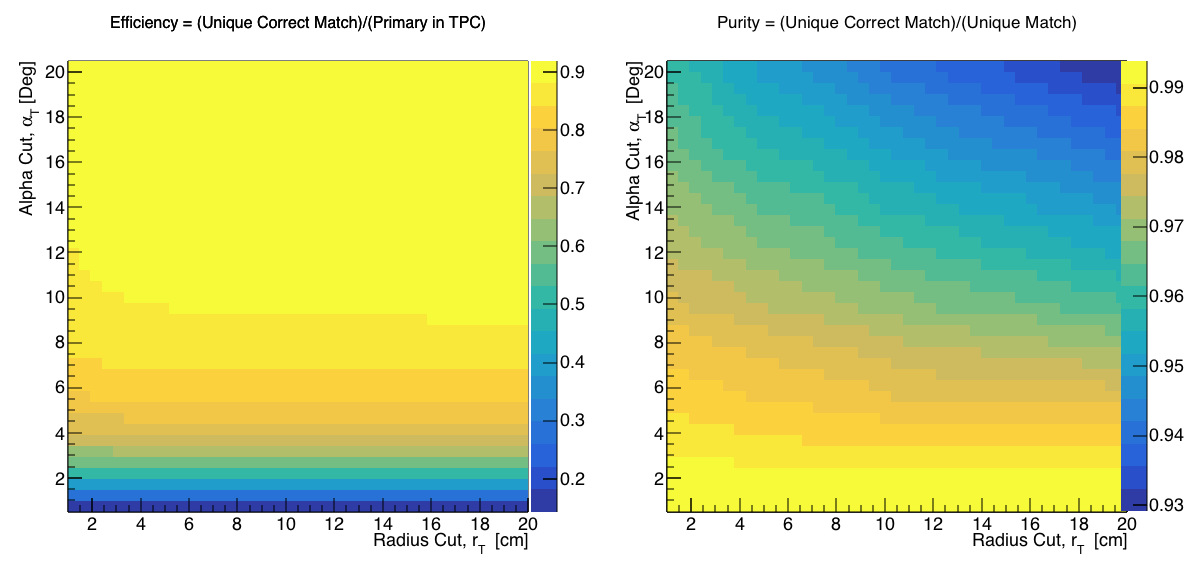
\includegraphics[width=15cm]{Chapter-5/Images/KEffPurity.png}
\caption{Efficiency (left) and purity (right) for WC2TPC match as a function of the radius and angle selections for the kaon sample.}
\label{fig:EffPurityK}
\end{figure}




\subsection{Tracking Optimization}\label{ch:TrackOptimization}
We perform an optimization of the clustering algorithm (see Section \ref{sec:SignalProc}) with the scope of maximizing the efficiency of finding the interaction point for the total hadronic cross section measurements. We define as the interaction point the most downstream point of a WC2TPC matched TPC tracks within the TPC fiducial volume. Since all the WC2TPC tracks are by definition beam particles, tracks travel from upstream to downstream in the TPC; thus, identifying the interaction point means to stop the tracking correctly. 

TrajCluster is the package used to cluster hits in LArIAT; this package counts more than 20 tunable parameters. A standard method to develop clustering algorithms and checking their performances is to ``hand scan", which means recognizing the effect of parameters tuning by looking at a series of data event displays. Albeit we recognize the importance of hand scanning as a great diagnosis tool, we developed a fully automated optimization package which compares MC reconstructed information to MC truth. 

We start by defining a figure of merit in order to discern what makes a parameter configuration better than an other. We chose the percentage of events whose reconstructed and true length differ less than 2 cm. In order to identify the true interaction point, no selection is performed on the scattering angle: even hadronic interaction flagged by Geant4 with very shallow angles (< 5$^\circ$) are kept to perform the optimization.
We then identify the parameters in TrajCluster that are most important to  correctly stop  the tracking and an appropriate range of values for each of them. We chose to optimize the parameters that leverage on the angle between consecutive groups of hits, the number of hits use in the cluster fit and the average hit charge to stop the tracking. We define a configuration space with all  possible combination of values for the chosen parameters and we perform reconstruction one combination at a time: the combination with the highest figure of merit determines the optimized tracking reconstruction.

We chose construct the combination space using a total of 5 parameters, 3 values each and two iterations of the method (for a total of 486 combinations). We run the combinations on a sample of 100000 pion events. 
After the optimization, the most upstream point of the tracking is correctly identified 99.5\% of the times, the most downstream point is correctly identified 62.5\% of the times, the tracking stops short about 15\% of the times and misses the interaction point 22.5\% of the times. Hand scanning confirmed that the missed interaction points happen in the vast majority of cases for very shallow angles, as shown in the event display in Figure \ref{evd:kink}, or in the case of angles visible only in one projection plane. We also noticed that the premature stopping of the tracks is often related to the presence of delta rays parallel to the track. We see room of improvement, such as the delta ray removal and a forced track breaking in case of a kink present in a single plane, for a future analysis. 

The procedure behind this optimization package is virtually applicable to any LArSoft module where it is possible to define figure of merit.


\begin{figure}[hpbt]
\centering
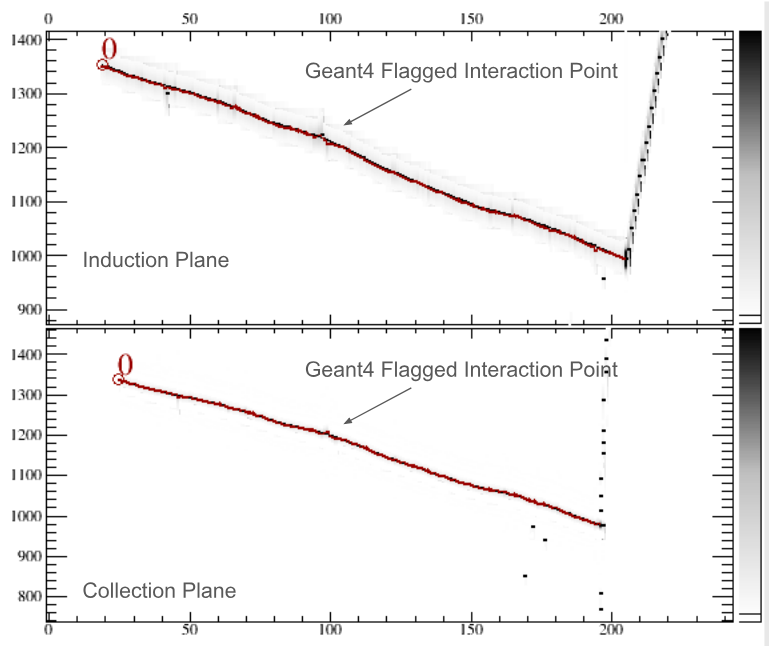
\includegraphics[width=15cm]{AppendixB-TrackingStudies/Kink.png}
\caption{Example of a shallow angle hadronic interaction ``missed" by the TrajCluster.}
\label{evd:kink}
\end{figure}

